%%%%%%%%%%%%%%%%%%%%%%%%%%%%%%%%%%%%%%%%%%%%%%%%%%%%%%
% A Beamer template for Ritsumeikan University       %
% Author: Ming-Hao Xu (Xu Minghao)                   %
% Date:   April 2022.                                %
% LPPL Licensed.                                     %
%%%%%%%%%%%%%%%%%%%%%%%%%%%%%%%%%%%%%%%%%%%%%%%%%%%%%%

\documentclass{beamer}
\usepackage{hyperref}

\usepackage[UTF8]{ctex}
\usepackage[T1]{fontenc}

% other packages
\usepackage{latexsym,amsmath,xcolor,multicol,booktabs,calligra}
\usepackage{graphicx,pstricks,listings,stackengine}
\usefonttheme[onlymath]{serif}

% dummy text; remove it when working on this template
\usepackage{lipsum}

\author{Ebola}
\title{计算几何4:平面最近点对、扫描线、辛普森积分}
\institute{
    Institute of Mathematics, \\
    Zhejiang University.
}
\date{Jan, 2024}
\usepackage{Ritsumeikan}

% defs
\def\cmd#1{\texttt{\color{red}\footnotesize $\backslash$#1}}
\def\env#1{\texttt{\color{blue}\footnotesize #1}}
\definecolor{deepblue}{rgb}{0,0,0.5}
\definecolor{deepred}{rgb}{0.6,0,0}
\definecolor{deepgreen}{rgb}{0,0.5,0}
\definecolor{halfgray}{gray}{0.55}

\lstset{
    basicstyle=\ttfamily\tiny,
    keywordstyle=\bfseries\color{deepblue},
    emphstyle=\ttfamily\color{deepred},    % Custom highlighting style
    stringstyle=\color{deepgreen},
    numbers=left,
    numberstyle=\small\color{halfgray},
    rulesepcolor=\color{red!20!green!20!blue!20},
    frame=shadowbox,
}


\begin{document}

\begin{frame}
    \titlepage
\end{frame}

\begin{frame}
    \tableofcontents[sectionstyle=show,subsectionstyle=show/shaded/hide,subsubsectionstyle=show/shaded/hide]
\end{frame}

\section{平面最近点对}

\begin{frame}{平面最近点对}
    \small 
    给定平面上 $n\;(\leq 4\times 10^5)$ 个点,求最近点对的距离。
    坐标范围:$[-10^7,10^7]$.

    \vspace{1em}
    请不要“充分发扬人类智慧”。
\end{frame}

\begin{frame}{平面最近点对}
    \footnotesize
    先介绍一种复杂度有保证的随机方法。

    \vspace{.5em}\pause
    设 $h$ 是前 $i$ 个点的最近点对距离。我们用 $h\times h$ 的网格来存储前 $i$ 个点(要用到哈希表)。
    显然,每个格子最多只有 $4$ 个点,否则最近点对距离一定小于 $h$。

    \begin{figure}[H]
        \centering
        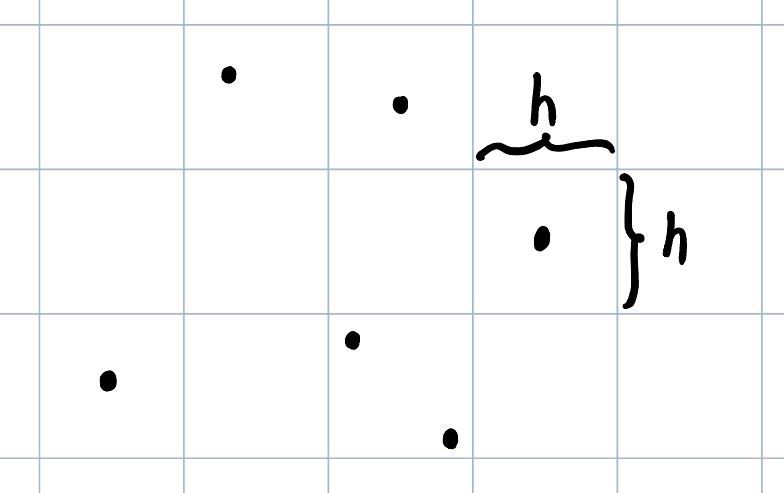
\includegraphics[width=0.5\textwidth]{pic/grid.jpg}
    \end{figure}

    现在,要求点 $i+1$ 和前 $i$ 个点之间的最近距离 $c$,只需要枚举点 $i+1$ 周围的九个格子
    即可,最多 $36$ 个点,是 $O(1)$ 的。

    \vspace{.5em}\pause
    如果 $c<h$,那么就要重构网格,重构网格的复杂度是 $O(i)$ 的。
    但如果先把所有点随机打乱,那么任何一个点 $i$ 是前 $i$ 个最近点对的概率是 $\frac{1}{i}$,
    所以期望复杂度 $\sum_{i=1}^n \frac{1}{i}O(i)=O(n)$.(常数巨大,甚至跑不过 $n\log n$)
\end{frame}

\begin{frame}{平面最近点对}
    \footnotesize
    现在来介绍 $n\log n$ 的方法。该方法基于分治。

    \vspace{.5em}\pause
    将所有点从左到右排序,分成两半;
    假如我们已经求出了两个点都在前一半的最近点对、两个点都在后一半的最近点对,
    其中较近的距离记为 $h$。现在我们要求第一个点在前一半、
    第二个点在后一半的最近点对。

    \vspace{.5em}\pause
    现在,假设直线 $x=x_m$ 是左右两部分的分界线,我们可以肯定,
    我们想求的点对一定在 $B$ 中:
    \begin{equation*}
        B=\{(x,y)\;|\;x_m-h\leq x\leq x_m+h\}.
    \end{equation*}

    \begin{figure}[H]
        \centering
        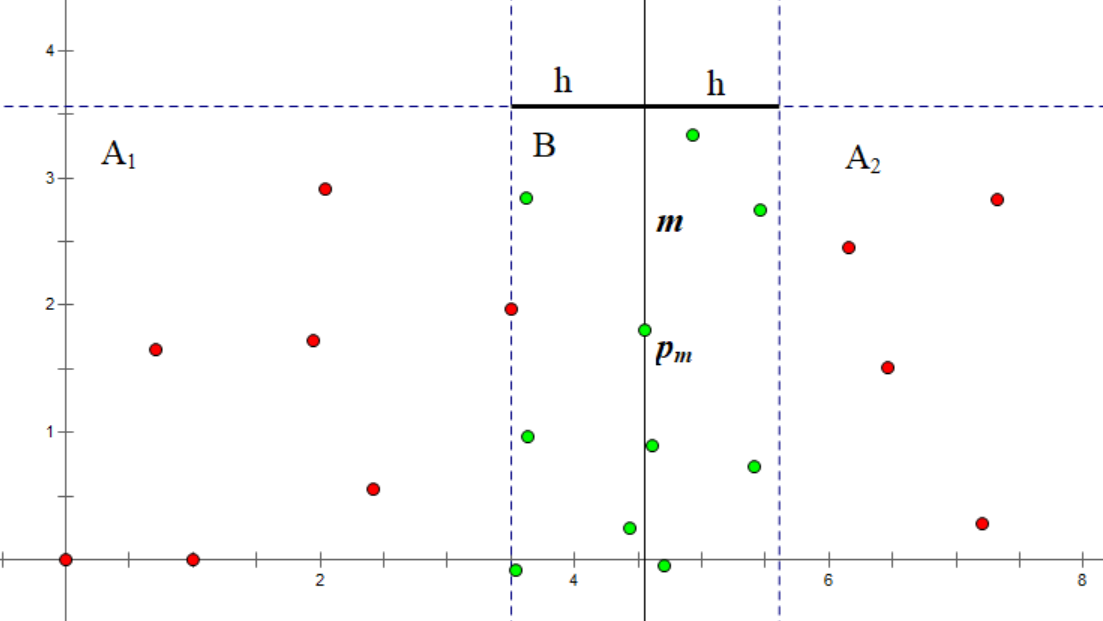
\includegraphics[width=0.7\textwidth]{pic/nearest-points1.png}
    \end{figure}
\end{frame}

\begin{frame}{平面最近点对}
    \footnotesize
    现在,我们来枚举 $B$ 中的点 $p_i$,
    我们想找到另一个 $B$ 中的点 $p_j$ 与它构成距离小于 $h$ 的最近点对,
    所以 $p_j$ 一定在 $C(p_i)$ 中:
    \begin{equation*}
        C(p_i)=\{p_j\;|\;p_j\in B \;\text{且}\; y_i-h \leq y_j \leq y_i\}.
    \end{equation*}
    (为了避免重复,我们只考虑纵坐标小于 $y_i$ 的那些点)

    \begin{figure}[H]
        \centering
        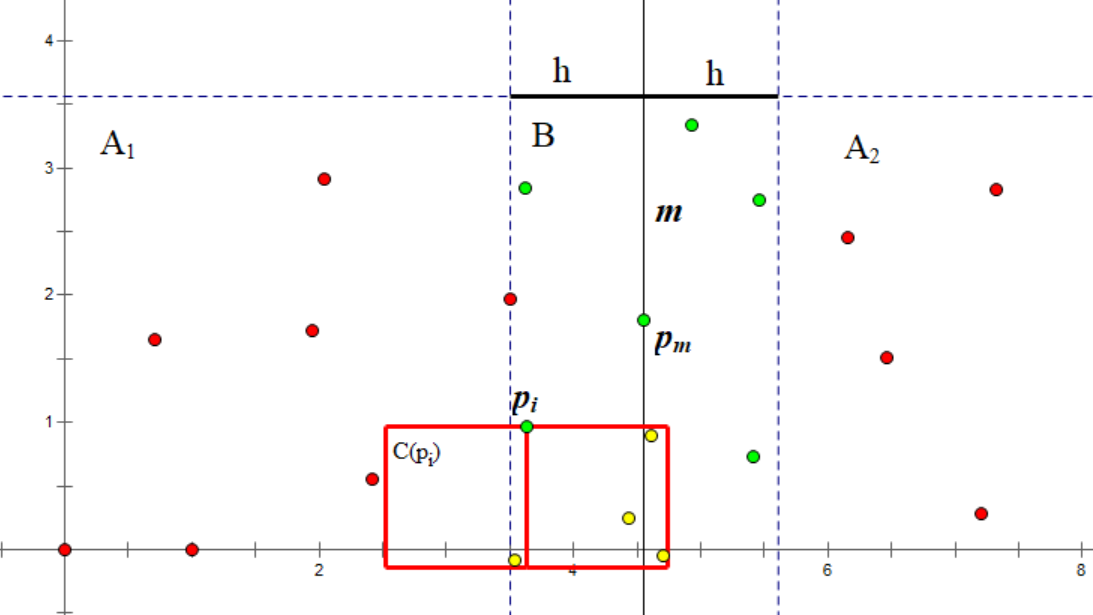
\includegraphics[width=0.7\textwidth]{pic/nearest-points2.png}
    \end{figure}
\end{frame}

\begin{frame}[fragile]{平面最近点对}
    \footnotesize
    现在,我们得到了分治的大致步骤:
    \begin{enumerate}
        \item 递归处理左右两个子问题,取较小值得到 $h$;
        \item 将区间内的所有点按纵坐标从小到大排序;
        \item 挑选出区域 $B$ 中的所有点;
        \item 枚举 $B$ 中的点 $p_i$,向前枚举 $p_j$ 并更新答案,直到 $y_j<y_i-h$。
    \end{enumerate}

    \vspace{1em}\pause
    如果用 \verb|sort| 来排序,复杂度会变成两个 $\log$,这样不好。
    但如果左右两个子区间分别按纵坐标排好了序,我们只要 $O(n)$ 二路归并就行了。

    \vspace{1em}
    现在只剩一个问题:第四步看起来可能会退化成 $O(n^2)$。
\end{frame}

\begin{frame}[fragile]{平面最近点对}
    \footnotesize
    我们把 $C(p_i)$ 的区域切割成 $8$ 个格子,如下图所示。

    \begin{figure}[H]
        \centering
        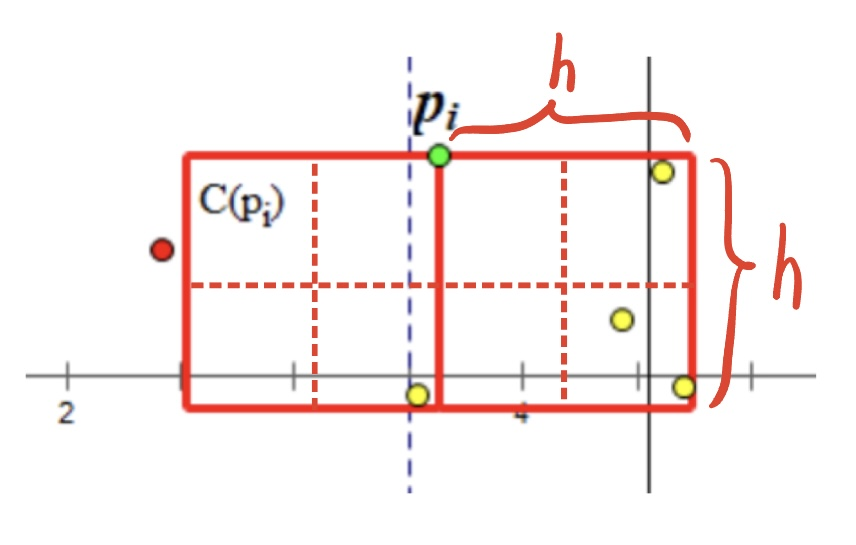
\includegraphics[width=0.5\textwidth]{pic/nearest-points3.jpg}
    \end{figure}

    \pause
    对于没有跨过分界线的格子,每个格子里最多只能有一个点,
    否则左侧的最近点对距离一定会 $<h$;
    同理,对于跨过分界线的格子,每个格子里最多只能有两个点。
    因此,$C(p_i)$ 中最多只有 $10$ 个点(不包括 $p_i$ 本身)。

    \vspace{1em}
    事实上,可以进一步证明: $C(p_i)$ 中最多只有 $7$ 个点(不包括 $p_i$ 本身)。
    不过不重要,总之我们知道了第四步中的 $j$ 循环最多跑常数次,
    因此合并过程的总复杂度是 $O(n)$ ,那么分治的总复杂度就是 $O(n\log n)$。
\end{frame}

\begin{frame}{平面最小周长三角形}
    \small
    在给定的一组点中,选择三个点,使得它们构成的三角形周长最小。
\end{frame}

\begin{frame}{平面最小周长三角形}
    \small
    做法和最近点对一样。分治,先找到两部分内部的最小周长三角形,
    记周长为 $d$,然后在区域 $B$ 中查找:
    \begin{equation*}
        B=\{(x,y)\;|\;x_m-\frac{d}{2}\leq x\leq x_m+\frac{d}{2}\}.
    \end{equation*}

    注意这里用了 $\frac{d}{2}$,因为周长为 $d$ 的三角形最长边一定小于 $\frac{d}{2}$.
    \pause 接下来一样的,在 $C(p_i)$ 中枚举 $p_j$ 和 $p_k$:
    \begin{equation*}
        C(p_i)=\{p_j\;|\;p_j\in B \;\text{且}\; y_i-\frac{d}{2} \leq y_j \leq y_i\}.
    \end{equation*}

    同样可以证明 $C(p_i)$ 中至多有常数个点,所以复杂度有保证。
\end{frame}

\begin{frame}{[CF120J] Minimum Sum}
    \small
    \begin{figure}[H]
        \centering
        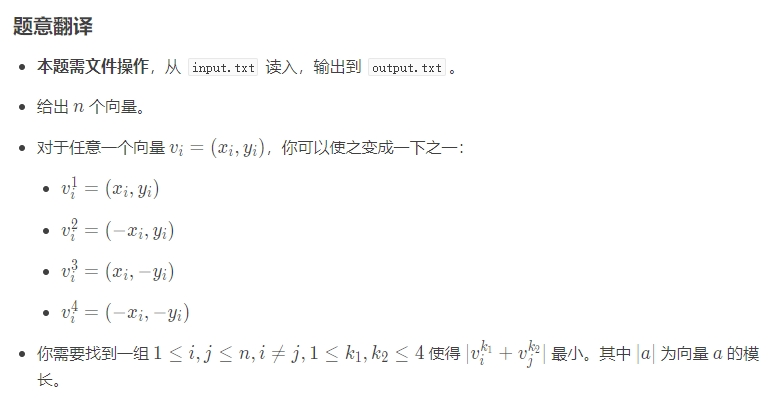
\includegraphics[width=\textwidth]{pic/minimumsum.png}
    \end{figure}
\end{frame}

\section{扫描线}

\begin{frame}{[POJ1151] Atlantis}
    \small
    给定平面上n个矩形,求被矩形覆盖区域的面积。
    \begin{figure}[H]
        \centering
        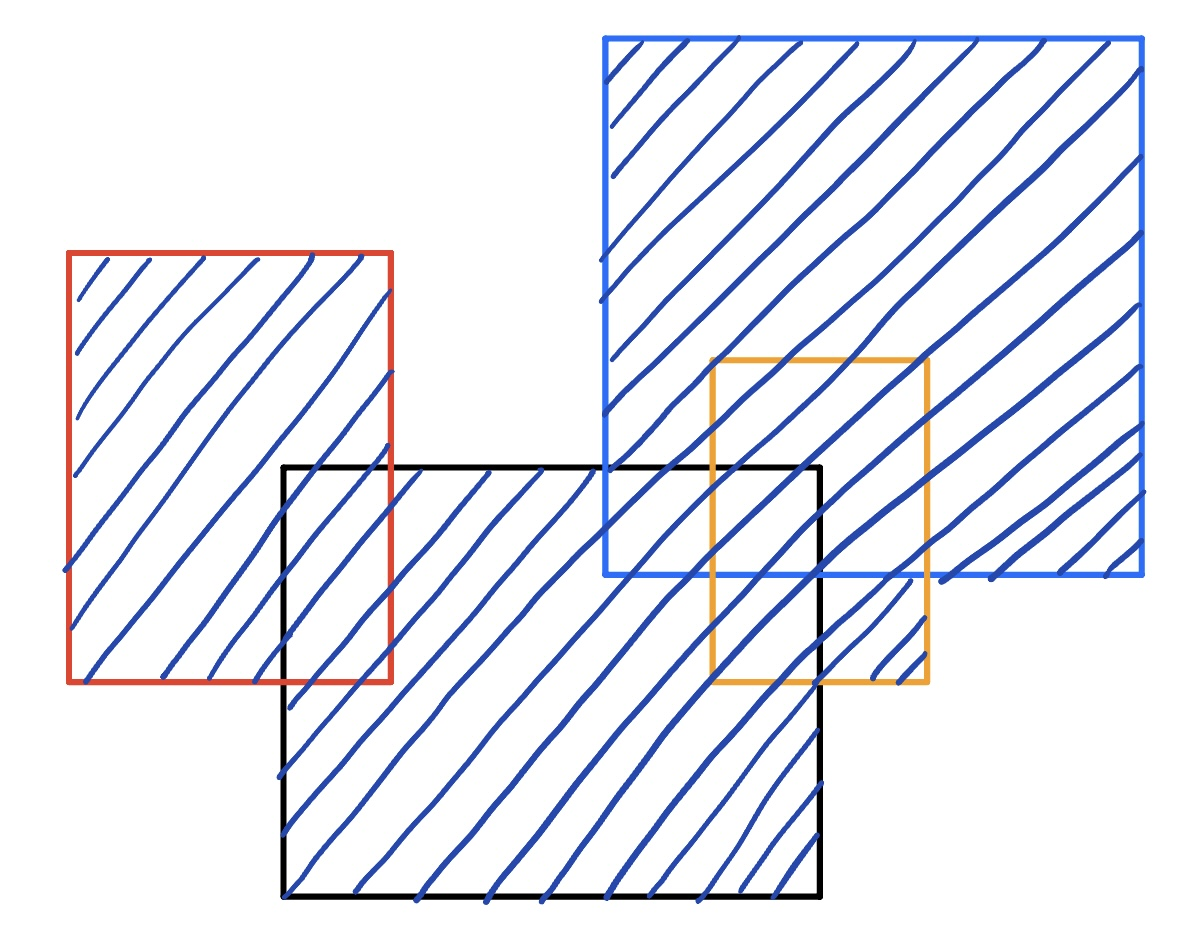
\includegraphics[width=0.6\textwidth]{pic/atlantis.jpg}
    \end{figure}
    $n\leq 100$,坐标范围 $[0,10^5]$.
\end{frame}

\begin{frame}{[POJ1151] Atlantis}
    \small
    我们想象一条从下往上走的水平直线,
    扫过矩形覆盖区域。
    (这里切出 ppt,手动播放动图 scanning.svg)

    \vspace{1em}\pause
    我们需要维护扫描线和矩形覆盖区域相交的部分,
    每当相交部分发生变化,
    就计算:相交部分的长度 $\times$ 上次发生变化的位置到现在的高度,
    这就是这一部分区域的面积。
    把每一部分面积加起来即得到答案。
\end{frame}

\begin{frame}{[POJ1151] Atlantis}
    \footnotesize
    如何维护扫描线和矩形覆盖区域相交的部分?
    
    \vspace{1em}\pause
    我们设数组 $a_1,...,a_m$,$a_i$ 表示扫描线的一小段 $[i,i+1)$ 和几个矩形相交。
    我们可以用线段树来维护这个数组。
    对于一个矩形 $[x_l,x_r]\times[y_l,y_r]$,当扫描线到达下边界 $y_l$ 时,
    就令 $a_{x_l},...,a_{x_r}$ 都加一;
    当扫描线到达上边界 $y_r$ 时,
    就令 $a_{x_l},...,a_{x_r}$ 都减一。
    可以用线段树的区间加来维护。

    \vspace{1em}\pause
    每个线段树节点需要记录自己所表示的线段中,非零部分的总长度。
    每次做加法时,如果当前节点表示的线段完全位于加法区间中,
    就打上区间 $+1$ 标记。
    向上合并时,如果有区间加法标记,非零部分长度就是线段长度,
    否则,就把左右儿子的非零部分总长度加起来。

    \vspace{1em}
    当然,扫描线也可以是从左往右扫的竖直直线,看个人习惯。
\end{frame}

\begin{frame}{值域离散化}
    \small
    如果坐标范围是 $[0,10^9]$ 怎么办?

    \vspace{1em}\pause
    离散化。把所有可能的横坐标按顺序排列成 $x_1,...,x_t$,
    然后建立 $[1,t]$ 的线段树。每次经过矩形边界要做加法时,
    先在所有横坐标中找到矩形顶点的横坐标 $x_i,x_j$,
    然后对 $[i,j]$ 进行区间加(或减)一。
    当然,统计线段 $[l,r]$ 的长度时,要用 $x_r-x_l$.
\end{frame}

\begin{frame}{[USACO5.5] 矩形周长Picture}
    \small
    给定若干个矩形,合并成一个图形,求周长。
    矩形数量 $\leq 5000$,坐标范围 $10^5$
    \begin{figure}[H]
        \begin{minipage}[t]{0.49\textwidth}
            \centering
            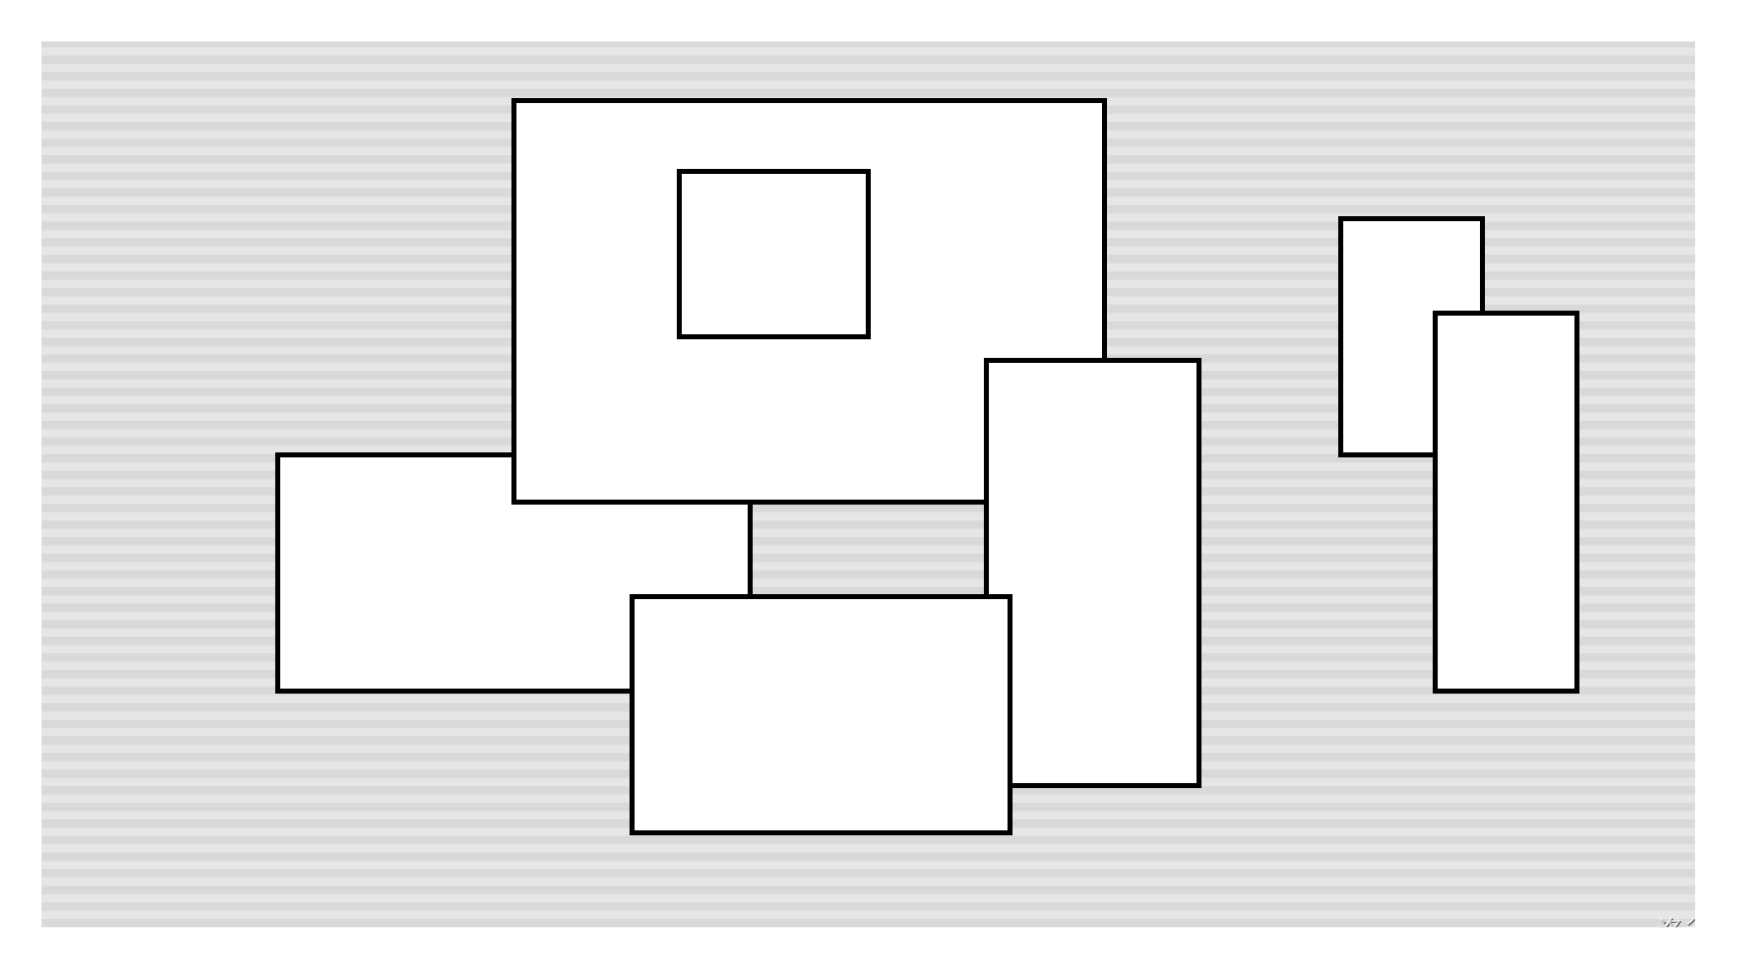
\includegraphics[width=\textwidth]{pic/picture-1.png}
        \end{minipage}
        \begin{minipage}[t]{0.49\textwidth}
            \centering
            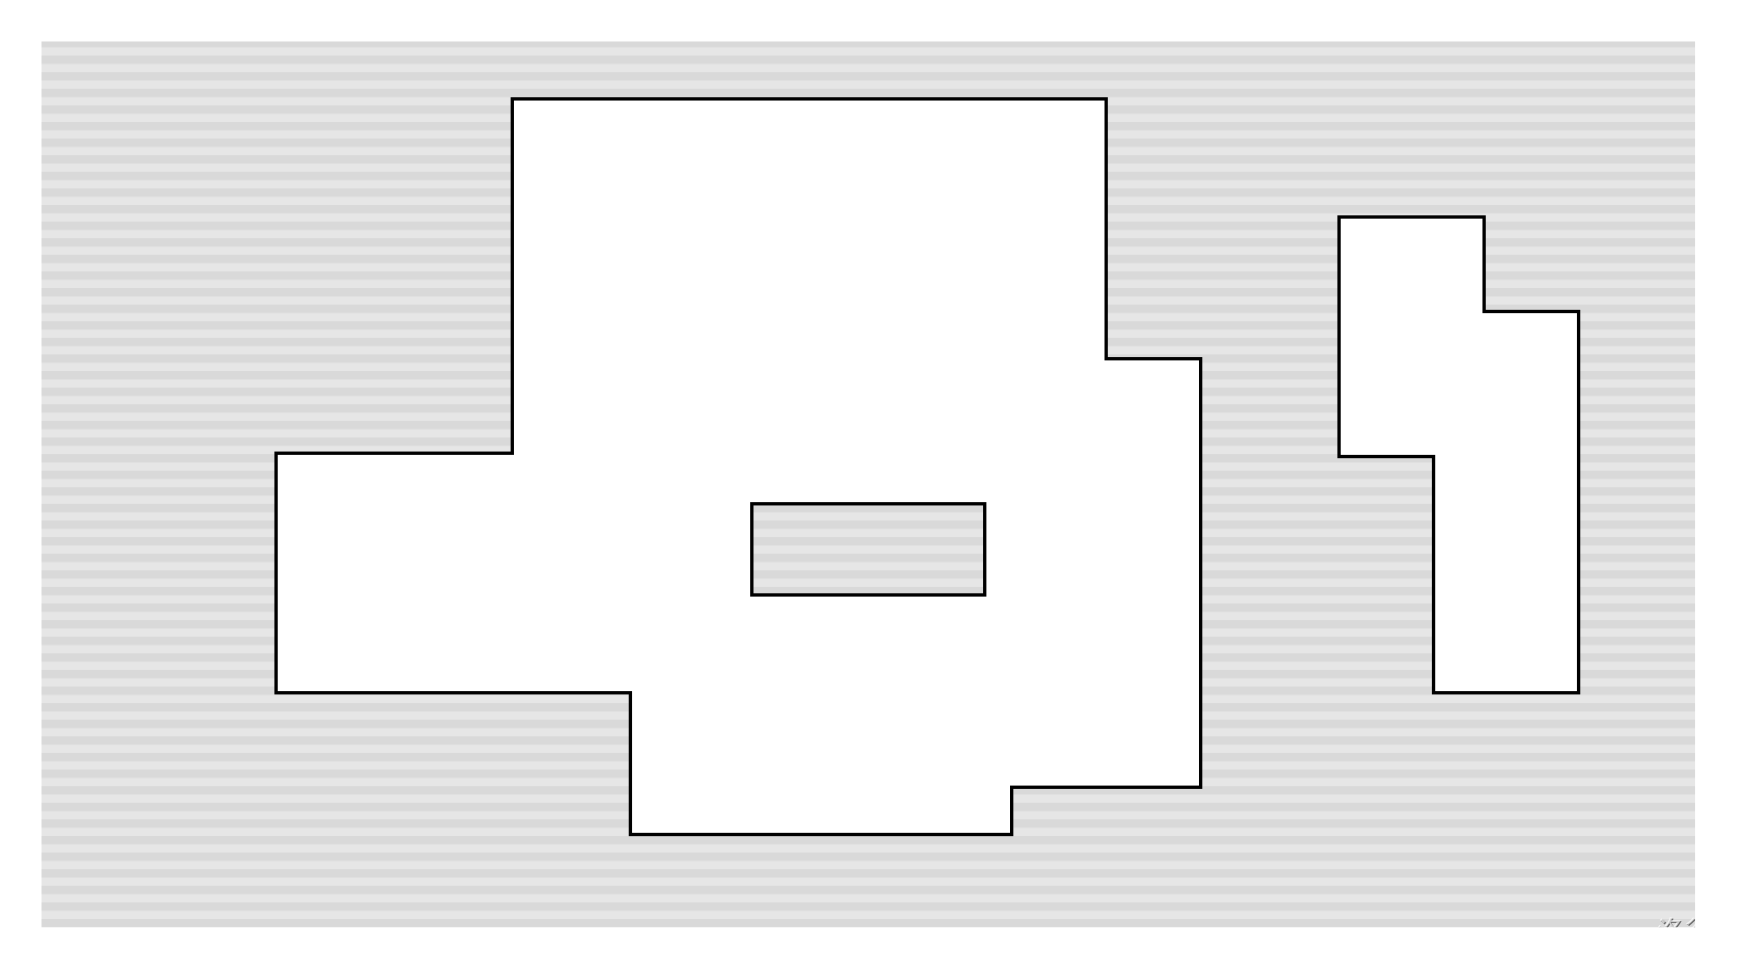
\includegraphics[width=\textwidth]{pic/picture-2.png}
        \end{minipage}
    \end{figure}
\end{frame}

\begin{frame}{[USACO5.5] 矩形周长Picture}
    \small
    我们把周长分成两个部分:横线的总长度、竖线的总长度。

    \vspace{1em}\pause
    对于横线的总长度,我们用一根水平直线从下往上扫描。
    如果 $y_i$ 和 $y_{i+1}$ 是相邻两个扫描高度(即扫描线发生变化的位置),
    扫描线在 $y_i$ 处和区域相交的长度是 $L_i$(注意,如果某个矩形的上边界在 $y_i$ 处,
    我们不算它和扫描线相交;如果下边界在 $y_i$ 处,则算它和扫描线相交),
    在 $y_{i+1}$ 处和区域相交的长度是 $L_{i+1}$,
    那么 $y_{i+1}$ 处露出来的横线长度就是 $|L_i-L_{i+1}|$(可以画图感受)。

    \vspace{1em}\pause
    竖线总长度同理,用竖直直线从左往右扫即可。
\end{frame}

\begin{frame}{[HNOI2012] 三角覆盖问题}
    \small
    求三角覆盖面积。
    
    \begin{figure}[H]
        \centering
        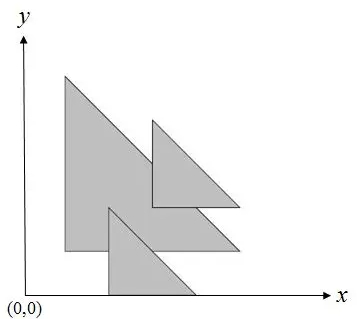
\includegraphics[width=0.6\textwidth]{pic/hnoi2012.png}
    \end{figure}
    
    三角形数量 $\leq 10^4$,坐标范围 $[0,10^6]$.
\end{frame}

\begin{frame}{[HNOI2012] 三角覆盖问题}
    \footnotesize
    从左到右\textbf{一格一格扫}。
    每到一个位置可能发生三种事情:线段上端点位置减一、增加一段新的线段、删除一个退化成点的线段。
    后两种事情总共发生 $O(n)$ 次,第一种事情会发生很多很多次,要优化。

    \vspace{1em}\pause
    如果某时刻一条线段被另一条完全覆盖,那么这条线段以后永远不会产生贡献,
    可以删去。(加入新线段时,把被它完全覆盖住的线段弹出;如果它自身被完全覆盖,则不添加之)
    最后得到的线段一定是下端点单调递增时,上端点也单调递增,可以用 set 维护。

    \vspace{1em}\pause
    当两线段相交时,下方线段上端点的改变并不会影响总覆盖长度。
    我们可以把它拆成:上方线段长度+下方线段长度-相交线段长度。
    这样,每一部分线段长度都是随着扫描线移动而减一的。
    用小根堆维护相交线段,当有相交线段退化成点时删去之。

    \vspace{1em}\pause
    这题暴力加各种优化其实可以过,数据很水,正解写起来细节非常多,
    大家量力而行。
\end{frame}

\begin{frame}{二维数点问题}
    \small
    给定平面上 $n\;(\leq 10^5)$ 个点 $(x_i,y_i)$,
    以及 $m\;(\leq 10^5)$ 个矩形 $[l_i,r_i]\times [d_i,u_i]$,
    问每个矩形包含了几个点(边界也算)。

    \vspace{1em}
    坐标范围 $[0,10^6]$(更大的话也可以离散化)。
\end{frame}

\begin{frame}{二维数点问题}
    \small
    一根线从左往右扫,碰到一个点就让位置 $y_i$ 加一;
    碰到矩形左边界,就让答案 $\text{ans}_i-=\text{sum}(d_i,u_i)$;
    碰到矩形右边界,就让答案 $\text{ans}_i+=\text{sum}(d_i,u_i)$。

    \vspace{1em}\pause
    注意当扫描线到达一个新位置时,正确的操作顺序应该是:处理左边界、处理加点、处理右边界。

    \vspace{1em}
    单点加、区间求和,用树状数组即可。
\end{frame}

\begin{frame}{[ARC077C] guruguru}
    \footnotesize
    给定一个数组 $a_1,...,a_n$ 和数字 $M$,
    从左到右依次操作,每次要把 $a_i$ 变成 $a_{i+1}$(不操作 $a_n$),
    可以使用如下两种操作:

    \begin{itemize}
        \item 令 $a_i$ 加一(当 $a_i=M$ 时,则令它变为 $1$);
        \item 直接令 $a_i=X$。
    \end{itemize}

    现在,请你确定 $X$,使总操作次数最少。
\end{frame}

\begin{frame}{[ARC077C] guruguru}
    \footnotesize
    可以将给定的数列看作若干个线段 $[a_i,a_{i+1}]$,若设定点在这个线段内(模意义下),则相当于可以从
    $a_i$ 跳到设定点,然后再一步一步走到 $a_{i+1}$,节省了 $x-a_i-1$ 步。
 
    \vspace{1em}\pause
    于是我们可以将所有线段按左端点排序,然后枚举设定点的位置。对于枚举到的位置,将包含它的线段全部加入即可。
    这相当于一个扫描线的过程,扫到一个点,将左端点位于该位置的线段全部加入,
    右端点位于该位置的线段全部删除。然后维护:当前加入的线段数量、当前能节省的总步数。
\end{frame}

\begin{frame}{[AH2017/HNOI2017] 影魔}
    \footnotesize

    奈文摩尔有 $n$ 个灵魂,他们在影魔宽广的体内可以排成一排,从左至右标号 $1$ 到 $n$。第 $i$ 个灵魂的战斗力为 $k_i$,灵魂们以点对的形式为影魔提供攻击力。对于灵魂对 $i, j\ (i<j)$ 来说,若不存在 $k_s\ (i<s<j)$ 大于 $k_i$ 或者 $k_j$,则会为影魔提供 $p_1$ 的攻击力。另一种情况,令 $c$ 为 $k_{i + 1}, k_{i + 2}, \cdots, k_{j -1}$ 的最大值,若 $c$ 满足:$k_i < c < k_j$,或者 $k_j < c < k_i$,则会为影魔提供 $p_2$ 的攻击力,当这样的 $c$ 不存在时,自然不会提供这 $p_2$ 的攻击力;其他情况的点对,均不会为影魔提供攻击力。

    \vspace{1em}
    影魔的挚友噬魂鬼在一天造访影魔体内时被这些灵魂吸引住了,他想知道,对于任意一段区间 $[a, b]$,位于这些区间中的灵魂对会为影魔提供多少攻击力,即考虑所有满足 $a\le i<j\le b$ 的灵魂对 $i, j$ 提供的攻击力之和。
    
    \vspace{1em}
    顺带一提,灵魂的战斗力组成一个 $1$ 到 $n$ 的排列:$k_1, k_1, \cdots, k_n$。
\end{frame}

\begin{frame}{[AH2017/HNOI2017] 影魔}
    \footnotesize
    换句话说:$(i,j)$ 产生 $p_1$ 贡献要求区间端点是最大值和次大值;
    产生 $p_2$ 贡献只要求区间某一个端点是最大值。

    \vspace{1em}
    对于一个位置 $i$,假设左右比它大的第一个位置分别为 $L_i$ 和 $R_i$,
    特别地,若右边没有比第 $i$ 个数大的数,则 $R_i=n+1$($L_i$同理)。
    考虑包含位置 $i$ 的点对产生多少贡献?

    \vspace{1em}\pause
    先考虑 $j>i$,显然当 $j>R_i$ 时不产生贡献;
    而 $(i,R_i)$ 的贡献是 $p_1$;
     $(i,i+1),(i,i+2),...,(i,R_i-1)$ 产生的贡献是 $p_2$。
    我们先把这类贡献加起来。

    \vspace{1em}\pause
    从右往左扫描线,每扫到一个位置 $i$,就对区间 $[i+1,R_i-1]$ 执行区间 $+p_2$ 操作;
    再给位置 $R_i$ 执行 $+p_1$ 操作(*);
    然后处理左端点在 $i$ 的询问,对询问区间 $[q_l,q_r]$ 进行求和,作为这部分的答案贡献给该询问。

    \vspace{1em}\pause
    现在考虑 $j<i$ 的部分,其实完全类似。但是我们刚刚挖了一个不大的坑……?

    \vspace{1em}\pause
    在考虑第二部分的时候,当扫到 $R_i$ 位置时,由于 $L_{R_i}<i$,所以 $(i,R_i)$ 被当成了一个
    贡献为 $p_2$ 的点对。这怎么办?

    \vspace{1em}\pause
    对,就在 (*) 的位置,把那个操作改成 $+(p_1-p_2)$ 就可以抵消了。
\end{frame}

\section{辛普森积分}

\begin{frame}{问题引入}
    给定一个函数$f(x)$和区间$[a,b]$,求
    \begin{equation*}
        \int_a^b f(x)\text{d}x
    \end{equation*}
    的近似值。
\end{frame}

\begin{frame}
    我们给出一个公式:
    \begin{equation*}
        I(a,b)=\frac{b-a}{6}\left(f(a)+4f\left(\frac{a+b}{2}\right)+f(b)\right)
    \end{equation*}
    
    假设$f(x)$是一个二次函数,那么恰好满足:
    \begin{equation*}
        \int_a^b f(x)\text{d}x=I(a,b)
    \end{equation*}

    如果$f(x)$不是二次函数呢?\pause
    我们可以计算$I(a,b),\;I\left(a,\frac{a+b}{2}\right),\;I\left(\frac{a+b}{2},b\right)$,如果
    \begin{equation*}
        \left|I(a,b)-\left(I\left(a,\frac{a+b}{2}\right)+I\left(\frac{a+b}{2},b\right)\right)\right| < \varepsilon
    \end{equation*}

    我们就认为我们的计算已经足够精确,将$I(a,b)$作为结果返回即可。否则,递归处理两个子区间。
\end{frame}

\begin{frame}[fragile]{代码}
    \begin{minipage}{\linewidth}
    \begin{lstlisting}[language=c++]
    double I(double l,double r)
    {
        double mid=(l+r)/2;
        return (F(l)+4*F(mid)+F(r))*(r-l)/6;
    }
    double simpson(double l,double r,double A)
    {
        double mid=(l+r)/2;
        double L=I(l,mid),R=I(mid,r);
        if(fabs(L+R-A)<eps) return L+R;
        return simpson(l,mid,L)+simpson(mid,r,R);
    }
    double simpson(double l,double r){return simpson(l,r,I(l,r));}
    \end{lstlisting}
    \end{minipage}
\end{frame}

\begin{frame}{[NOI2005] 月下柠檬树}
    求一棵由圆台、圆锥组成的树在平行光下的投影面积。

    \begin{figure}[H]
        \begin{minipage}[t]{0.49\textwidth}
            \centering
            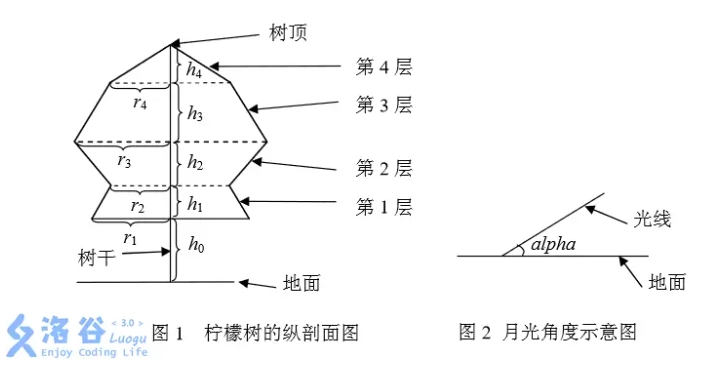
\includegraphics[width=\textwidth]{pic/noi2005.png}
        \end{minipage}
        \begin{minipage}[t]{0.49\textwidth}
            \centering
            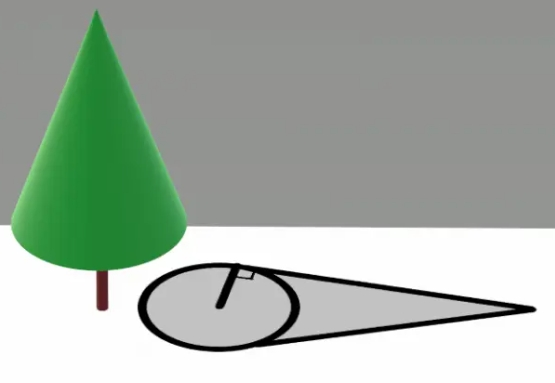
\includegraphics[width=\textwidth]{pic/noi2005-2.png}
        \end{minipage}
    \end{figure}

\end{frame}

\begin{frame}{[NOI2005] 月下柠檬树}
    \footnotesize
    \begin{figure}[H]
        \centering
        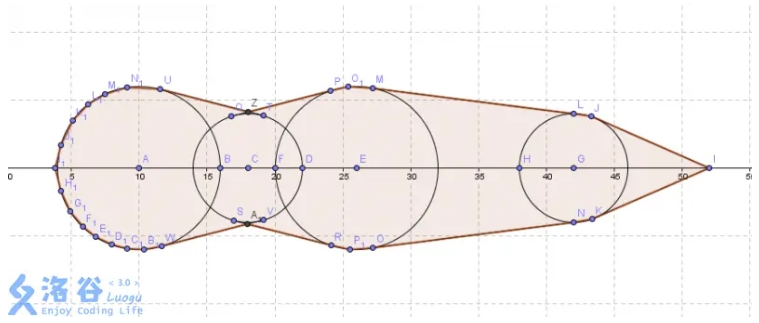
\includegraphics[width=0.9\textwidth]{pic/noi2005-3.png}
    \end{figure}

    根据光线角度算出所有圆的圆心坐标,再算出相邻两个圆的公切线。
    注意:如果在投影里,一个圆被旁边的圆完全包含,则应该跳过之。
    把所有的圆存好、所有的公切线成对存好。

    \vspace{.5em}\pause
    接下来用辛普森积分求面积,我们只需要解决直线 $x=t$ 与图形相交部分的长度。
    因为图形是一个单连通区域,我们可以枚举所有圆,求它与圆相交部分的长度;
    再枚举所有成对的公切线,求它被两条公切线夹住部分的长度;
    最后把求得的长度取最大值,就是和图形相交部分的长度。
\end{frame}

\begin{frame}
    \begin{center}
        {\Huge\calligra Thank You}
    \end{center}
\end{frame}

\end{document}